\section{Methods}\label{sec:methods}

\subsection{Model Architecture}

The input image is split into non-overlapping $4\times4$ patches via a strided Conv2d (the \emph{patch embedding}), producing 64 tokens of dimension 192.
A learnable \texttt{[CLS]} token is prepended, positional embeddings are added, and the resulting 65-token sequence passes through 9 Pre-LN transformer encoder blocks~\cite{dosovitskiy2021vit}.
Each block applies multi-head self-attention (4 heads, dimension 192) followed by a two-layer MLP (hidden dimension 768), both with residual connections.
The \texttt{[CLS]} output at the final block feeds a linear classification head producing 10 logits.
Total trainable parameters: 4{,}028{,}170.

Under the strong recipe, \textbf{stochastic depth} (DropPath~\cite{huang2016deep}) is applied to both residual paths in each block, with rate linearly scaled from 0 to 0.1 across the 9 blocks.
This encourages each block to contribute independently rather than relying on the residual stream, acting as a structured dropout over depth.

\begin{figure}[ht]
    \centering
    \small
    \begin{tabular}{ll}
        \toprule
        Hyperparameter  & Value                   \\
        \midrule
        Image size      & $32\times32$            \\
        Patch size      & $4\times4$ (64 patches) \\
        Embedding dim   & 192                     \\
        Depth           & 9 blocks                \\
        Attention heads & 4 (head dim 48)         \\
        MLP ratio       & 4.0 (hidden 768)        \\
        Dropout         & 0.1                     \\
        Parameters      & 4{,}028{,}170           \\
        \bottomrule
    \end{tabular}
    \captionof{table}{ViT configuration used in all experiments.}\label{tab:vit-config}
\end{figure}

\subsection{Adapting the Four CNN Tricks to ViT}

Each trick was originally designed for the CNN in~\cite{garg2024cifar10}.
We describe each trick, its rationale in the CNN context, and how we adapted it.

\paragraph{Frozen patch-whitening initialisation.}
In the CNN, the first convolutional layer is initialised with whitened PCA filters of the training-set patch covariance, then frozen.
The intent is to provide a rotation-invariant, decorrelated input representation from epoch 0, allowing subsequent layers to focus on learning discriminative features.

We apply the same procedure to the ViT's $4\times4$ Conv2d patch embedding.
Let $\mathbf{\Sigma} = \mathbf{P}^\transpose \mathbf{P}/N$ be the covariance of all $3\times4\times4 = 48$-dimensional patches from the first 5{,}000 training images.
Eigendecomposition gives $\mathbf{\Sigma} = \mathbf{V} \mathbf{\Lambda} \mathbf{V}^\transpose$, and the whitening filters are:
\begin{equation}
    \mathbf{w}_k = -\mathbf{w}_{k+D} =
    \frac{\mathbf{v}_k}{\sqrt{\lambda_k + \varepsilon}},
    \quad k=1,\dots,D,
\end{equation}
filling the first 96 of 192 embedding channels with positive/negative pairs.
The remaining 96 channels retain He initialisation.
The embedding is then frozen for the full training run.

\paragraph{Dirac/identity initialisation.}
In the CNN, the first $C_\text{in}$ filters of each grouped-convolution block are set to the Dirac delta, initialising them as near-identity maps.
This is designed to ensure each block starts as a pass-through, with deviation from the identity learned progressively.

We adapt this to the QKV and output projections of every attention block.
Each of the three $D \times D$ sub-matrices of $\mathbf{W}_\text{QKV} \in \R^{3D \times D}$ is set to $\mathbf{I}_D$, and $\mathbf{W}_O \in \R^{D \times D}$ is set to $\mathbf{I}_D$.
We also test a \emph{soft} variant: $\mathbf{W} \leftarrow \alpha \mathbf{I} + \left( 1 - \alpha \right) \mathbf{W}_\text{rand}$ at $\alpha = 0.3$, blending identity and standard random initialisation.

\paragraph{ScaleBias + Lookahead.}
The CNN appends a fixed \texttt{Scale (1/9)} module after global max-pooling over a $3\times3$ spatial map.
The factor $1/9$ normalises the sum of 9 pooled values.
We generalise to a learnable per-feature affine transform $y_i = s_i x_i + b_i$ (ScaleBias) initialised at $s_i{=}1/9$, replacing the linear head.
The ViT has no analogous pooling (the \texttt{[CLS]} output is a single vector), so the $1/9$ factor is architecturally unmotivated.

Lookahead~\cite{zhang2019lookahead} wraps the base optimiser (AdamW) with a slow-weight update:
\begin{equation}
    \phi_{t+k} \gets \phi_t + \alpha \left( \theta_{t+k} - \phi_t \right),\quad
    \theta \gets \phi_{t+k},
\end{equation}
with $k = 6$, $\alpha = 0.5$.
In the strong recipe we use $s_i = 1.0$ and a cosine LR schedule instead of {OneCycleLR}.

\paragraph{Alternating flip.}
Instead of random horizontal flip (independent Bernoulli ($p{=}0.5$) per sample), we deterministically flip every odd-indexed sample, guaranteeing exactly 50\% flipped images in every epoch with zero batch-level flip-count variance.
The motivation is to reduce gradient noise from inconsistent flip counts within a batch.

Figure~\ref{fig:flip-comparison} illustrates the difference.
In random flip (left), the flip decision is re-drawn each epoch, so the same image may be flipped in one epoch and not the next, and the number of flips per batch varies.
In alternating flip (right), each image has a fixed parity: odd-indexed images are always flipped, even-indexed images are never flipped.
Every epoch and every batch sees exactly the same flip assignment, eliminating the stochastic component entirely.

\begin{figure}[h]
    \centering
    \begin{subfigure}[t]{0.48\linewidth}
        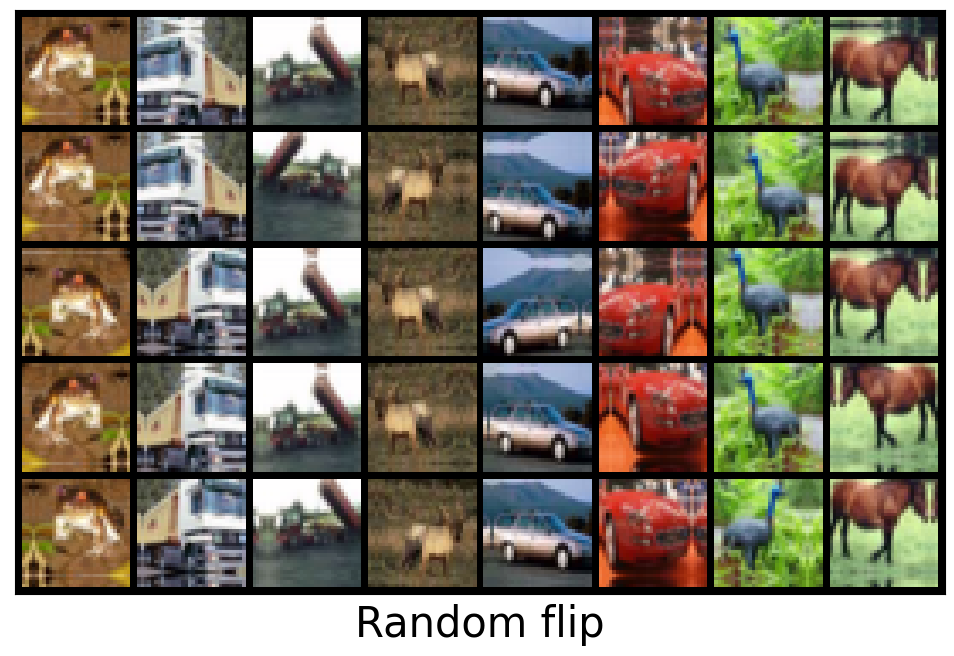
\includegraphics[width=\linewidth]{figures/random_flip.png}
        \caption{Random flip: flip decisions are re-sampled each epoch, producing variable flip patterns across rows.}\label{fig:random-flip}
    \end{subfigure}
    \hfill
    \begin{subfigure}[t]{0.48\linewidth}
        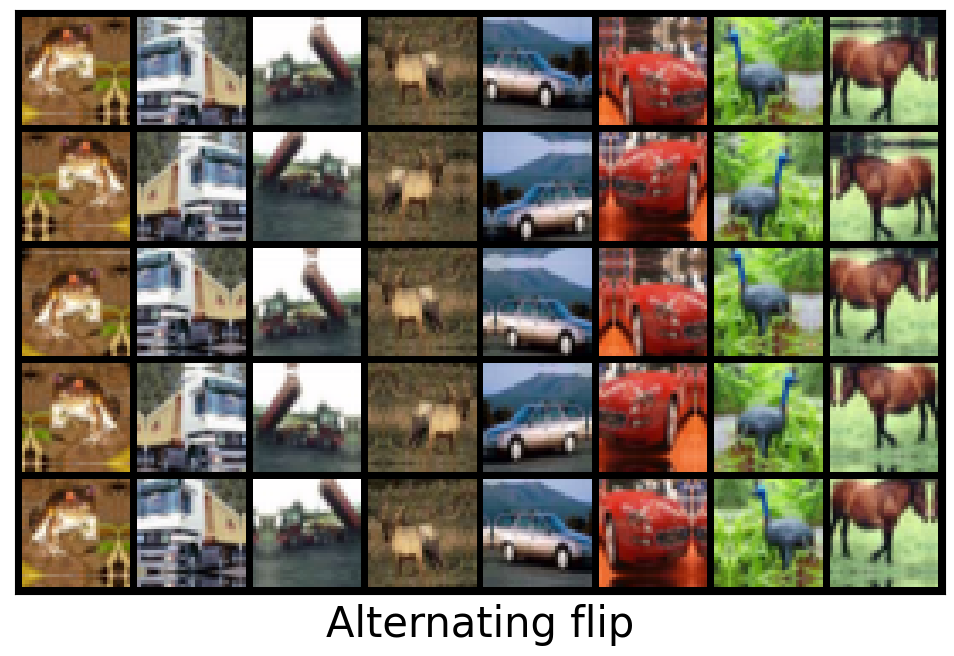
\includegraphics[width=\linewidth]{figures/alternating_flip.png}
        \caption{Alternating flip: each image has a fixed odd/even assignment that repeats identically every epoch.}\label{fig:alt-flip}
    \end{subfigure}
    \caption{Random flip (left) vs.\ alternating flip (right) over five epochs on the same eight \cifar{} images (columns = images, rows = epochs). Random flip produces inconsistent patterns; alternating flip is deterministic and identical across epochs.}\label{fig:flip-comparison}
\end{figure}

\subsection{Training Recipes}

\begin{table}[h]
    \centering
    \setlength{\tabcolsep}{3pt}
    \small
    \begin{tabular}{lll}
        \toprule
        Hyperparameter & Weak             & Strong                          \\
        \midrule
        Epochs         & 100              & 300                             \\
        Peak LR        & $3\times10^{-4}$ & $1\times10^{-3}$                \\
        LR schedule    & OneCycleLR       & Cosine + 5\% warmup             \\
        DropPath       & ---              & 0.1 (linear)                    \\
        Augmentation   & Crop + flip      & Crop + flip + RandAugment       \\
        Mixup / CutMix & ---              & $\alpha{=}0.8$ / $\alpha{=}1.0$ \\
        \bottomrule
    \end{tabular}
    \caption{Training recipe comparison. Both use AdamW, batch size 256, weight decay 0.05, label smoothing 0.1, AMP float16.}\label{tab:recipes}
\end{table}

The weak recipe provides a controlled, low-variance environment for isolating each trick's effect, comparable to the CNN's own training regime.
The strong recipe pushes accuracy to the level achievable with current best-practice ViT training, testing whether the tricks remain useful at the higher baseline.

